%Subsection{extension}
%lensed_waveguide_extension
Beside the previous discussion about the lensed waveguide, there are more operations we can resort to. From \cite{integrated_coupling_between_LD_SMF} we can come to more ideas to promote the coupling efficiency between TLF and lensed waveguide. The author at the end has presented a tapered core fiber like Fig.\ref{fig:tapered_core_fiber}, which is capable to confine more beam rays. From this we also get to know there is a small distance $h_{1}$ between the lens end $H_{1}$ and core interface $H_{2}$ because the lens end is not the exact minimum spot location for a lensed waveguide. Thus it is possible to gain a higher coupling efficiency if we expand properly the distance between the lens and the core within the lensed waveguide as a 'neck' between the lens and the waveguide (see Fig. \ref{fig:lensed_waveguide_neck}). For a proper 'neck' length $h_{1}$ higher coupling efficiency should be achieved. This setup will be considered at further development instead of in this work.
\begin{figure}[!ht]
\centering
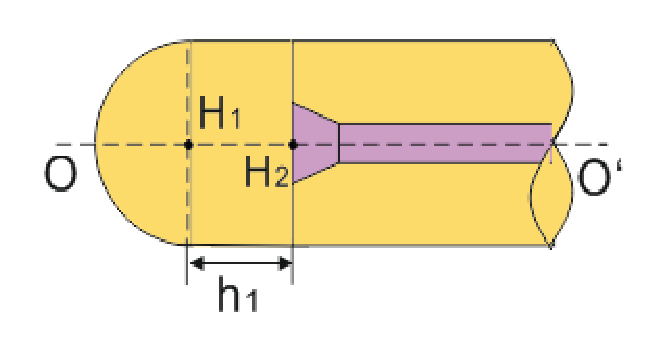
\includegraphics[width=0.7\textwidth]{bilder/tapered_core_fiber}
\caption {Schema of tapered core fiber\cite{integrated_coupling_between_LD_SMF}.}
\label{fig:tapered_core_fiber}
\end{figure}
\begin{figure}[!ht]
\centering
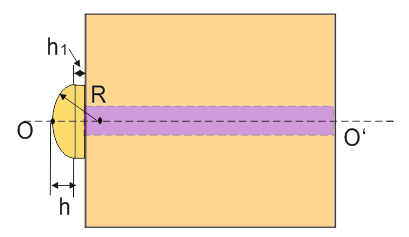
\includegraphics[width=0.7\textwidth]{bilder/lensed_waveguide_neck}
\caption {Schema of a lensed buried waveguide with a 'neck'.}
\label{fig:lensed_waveguide_neck}
\end{figure}
